\chapter{Experimental Validation of Proposed Methods}
\label{chap:experiments}

This chapter presents the experimental evaluation of both proposed frameworks. Section~\ref{sec:bf_experiments} validates BackFlush through four research questions addressing state-of-the-art comparison, trigger generalization, detection mechanism, and unlearning dynamics. Section~\ref{sec:rp_experiments} validates RePAIR through three research questions addressing baseline comparison, end-to-end pipeline effectiveness, and qualitative behavior, followed by a set of ablation studies.


%% ============================================================
\section{BackFlush: Backdoor Detection and Elimination}\label{sec:bf_experiments}
%% ============================================================

We evaluate BackFlush through four research questions. \textbf{(RQ1)} Does BackFlush outperform state-of-the-art defenses in backdoor removal while preserving watermarks? \textbf{(RQ2)} Does it generalize across diverse trigger types without prior knowledge? \textbf{(RQ3)} Does Backdoor Susceptibility Amplification enable bounded-time detection? \textbf{(RQ4)} How does RoPE achieve effective unlearning without degrading model utility?

%% ------------------------------------------------------------
\subsection{Experimental Setup}\label{subsec:bf_setup}
%% ------------------------------------------------------------

\noindent
\textbf{Benchmarks and Models.} We compare BackFlush against seven baselines, namely Fine-Mixing~\citeauthor{zhang2022fine} BEEAR~\citeauthor{zeng2024beear} Model-Merging~\citeauthor{arora2024here} Information Conflicts~\citeauthor{chen2024neutralizing} LocPhylax~\citeauthor{lin2025backdoor} SANDE~\citeauthor{li2025simulate} and W2SDefense~\citeauthor{zhao2025unlearning} We use TriviaQA~\citeauthor{joshi2017triviaqa} as $\mathcal{D}_{\textit{benign}}$, SciQ~\citeauthor{welbl2017crowdsourcing} as $\mathcal{D}_{\textit{aux}}$, and TinyStories~\citeauthor{eldan2023tinystories} for utility evaluation. For detection, we construct $\mathcal{D}_{\textit{probe}}$ with synthetic triggers. Triggers include repeated words, typos, patterns, and phrases, while payloads contain hate speech, violence-provoking statements, sentiments, and misinformation, with examples shown in Table~\ref{tab:poison_samples}. We test on three architectures to evaluate generalization, namely Qwen2.5-1B-Instruct~\citeauthor{qwen2.5} Llama-3.2-1B-Instruct~\citeauthor{grattafiori2024llama} and Mistral-7B-Instruct~\citeauthor{jiang2023mistral7b}

\medskip
\noindent
\textbf{Metrics.} We evaluate using four metrics. The first is \textit{Clean Accuracy (CACC)}, the percentage of clean samples correctly predicted without triggers, where higher is better. The second is \textit{Attack Success Rate (ASR)}, the percentage of poisoned samples exhibiting malicious triggered responses, where lower is better. The third is \textit{Utility}, model performance measured by perplexity on TinyStories~\citeauthor{eldan2023tinystories} where lower is better. The fourth is \textit{Watermark Verification}, a binary indicator $\mathcal{S}(\mathcal{M}, k) \in \{0, 1\}$ of watermark preservation, where T denotes preserved and F denotes failed.


%% ------------------------------------------------------------
\subsection{RQ1: Comparison with State-of-the-Art}\label{subsec:bf_rq1}
%% ------------------------------------------------------------

Table~\ref{tab:defense_comparison} presents the performance comparison across three LLM architectures. \colorbox{green!30}{Green} highlights indicate best performance and \colorbox{yellow!40}{yellow} indicates second-best. BackFlush-GA and BackFlush-RoPE consistently rank first or second across all metrics.

\begin{table}[htbp]
\centering
\caption{Performance comparison of backdoor defense methods across three LLM architectures. Lower values are better for ASR ($\downarrow$) and Utility ($\downarrow$), while higher values are better for CACC ($\uparrow$) and W/M.}
\label{tab:defense_comparison}
\footnotesize
\renewcommand{\arraystretch}{1.25}
\setlength{\tabcolsep}{3.5pt}
\begin{adjustbox}{max width=\textwidth}
\begin{tabular}{p{2.6cm}|cccc|cccc|cccc}
\Xhline{1.15pt}
\multirow{2}{*}{\textbf{Method}} &
\multicolumn{4}{c|}{\textbf{Mistral-7B}} &
\multicolumn{4}{c|}{\textbf{Llama-3-8B}} &
\multicolumn{4}{c}{\textbf{Qwen-2.5-7B}} \\
\cmidrule(lr){2-5}\cmidrule(lr){6-9}\cmidrule(lr){10-13}
& \textbf{ASR}$\downarrow$ & \textbf{CACC}$\uparrow$ & \textbf{Util}$\downarrow$ & \textbf{W/M}
& \textbf{ASR}$\downarrow$ & \textbf{CACC}$\uparrow$ & \textbf{Util}$\downarrow$ & \textbf{W/M}
& \textbf{ASR}$\downarrow$ & \textbf{CACC}$\uparrow$ & \textbf{Util}$\downarrow$ & \textbf{W/M} \\
\Xhline{1.15pt}
Base
& 93.60 & 98.32 & 5.73 & T
& 93.27 & 95.49 & 5.83 & T
& 98.53 & 91.32 & 5.50 & T \\
\midrule
Fine-Mixing
& 27.77 & 80.59 & 16.14 & F
& 27.10 & 93.13 & 13.37 & F
& 35.13 & 90.17 & 10.28 & F \\
\rowcolor{gray!15}
BEEAR
& 30.48 & 91.01 & 10.58 & T
& 33.47 & 90.66 & 10.01 & T
& 30.00 & 89.01 & 11.32 & T \\
IC
& 35.84 & 98.47 & \colorbox{yellow!40}{8.37} & F
& 50.13 & 93.27 & 11.19 & F
& 43.13 & 93.17 & 9.13 & F \\
\rowcolor{gray!15}
Model-Merging
& 20.23 & 99.03 & 15.12 & F
& 25.11 & 92.47 & 15.17 & F
& 27.18 & \colorbox{green!30}{96.98} & 13.10 & F \\
SANDE
& 47.13 & \colorbox{yellow!40}{99.17} & 9.16 & F
& 49.03 & 96.13 & 13.13 & F
& 57.17 & 85.01 & 12.10 & F \\
\rowcolor{gray!15}
LocPhylax
& 13.28 & 98.10 & 10.59 & T
& 27.12 & 87.77 & \colorbox{yellow!40}{9.13} & T
& 22.88 & 90.13 & \colorbox{yellow!40}{8.73} & T \\
W2SDefense
& 44.44 & 89.13 & 11.64 & F
& 60.00 & \colorbox{yellow!40}{97.13} & 10.19 & F
& 50.13 & \colorbox{yellow!40}{95.13} & 11.10 & F \\
\midrule\midrule
\textbf{BackFlush-GA}
& \colorbox{yellow!40}{1.36} & \colorbox{green!30}{99.68} & 10.52 & F
& \colorbox{yellow!40}{2.13} & \colorbox{green!30}{99.08} & 11.37 & F
& \colorbox{yellow!40}{2.27} & 93.27 & 9.16 & F \\
\textbf{BackFlush-RoPE}
& \colorbox{green!30}{0.98} & 98.58 & \colorbox{green!30}{6.39} & T
& \colorbox{green!30}{0.83} & 97.04 & \colorbox{green!30}{7.28} & T
& \colorbox{green!30}{0.73} & 90.19 & \colorbox{green!30}{6.13} & T \\
\Xhline{1.15pt}
\end{tabular}
\end{adjustbox}
\end{table}

\subsubsection{Attack Success Rate Analysis}

As anticipated from the method design in Chapter~\ref{chap:method}, injecting $\mathcal{D}_{\textit{aux}}$ and subsequently removing it using BackFlush-RoPE and BackFlush-GA achieved the lowest ASR across all architectures (Table~\ref{tab:defense_comparison}), with 0.98\% and 1.36\% respectively on Mistral-7B. Among baselines, SANDE~\citeauthor{li2025simulate} assumes identical payloads, achieving 47.13\% ASR on Mistral-7B. BEEAR~\citeauthor{zeng2024beear} failed to identify several trigger types. Fine-Mixing~\citeauthor{zhang2022fine} using a 1:4 interpolation ratio resulted in approximately 25\% ASR. Model-Merging~\citeauthor{arora2024here} achieved approximately 25\% ASR. Information Conflicts~\citeauthor{chen2024neutralizing} achieved approximately 25\% ASR. LocPhylax~\citeauthor{lin2025backdoor} removed most backdoors incompletely, with 13--27\% residual ASR. W2SDefense~\citeauthor{zhao2025unlearning} achieved approximately 44\% ASR. This behavior is consistent across all three architectures, confirming that BackFlush's advantage is architecture-independent.

\subsubsection{Watermark Preservation}

SANDE~\citeauthor{li2025simulate} Fine-Mixing~\citeauthor{zhang2022fine} Model-Merging~\citeauthor{arora2024here} Information Conflicts~\citeauthor{chen2024neutralizing} W2SDefense~\citeauthor{zhao2025unlearning} and BackFlush-GA all failed to maintain watermark signatures (W/M = F). In contrast, BEEAR~\citeauthor{zeng2024beear} LocPhylax~\citeauthor{lin2025backdoor} and BackFlush-RoPE preserved watermarks (W/M = T). This confirms that RoPE's bounded rotation loss preserves watermark parameters while GA's unbounded gradients corrupt them. Critically, among watermark-preserving methods, only BackFlush-RoPE also achieves effective backdoor removal with ASR below 1\%, while BEEAR and LocPhylax retain 13--33\% residual ASR. This behavior is consistent across all architectures.

\subsubsection{Clean Accuracy Analysis}

Removing backdoors while maintaining clean performance is critical. SANDE~\citeauthor{li2025simulate} Model-Merging~\citeauthor{arora2024here} and LocPhylax~\citeauthor{lin2025backdoor} achieve near-ideal CACC of approximately 99\%, while Fine-Mixing~\citeauthor{zhang2022fine} W2SDefense~\citeauthor{zhao2025unlearning} BEEAR~\citeauthor{zeng2024beear} and Information Conflicts~\citeauthor{chen2024neutralizing} degrade to approximately 80--93\%. BackFlush-RoPE and BackFlush-GA exceed baseline CACC at approximately 99\%, as backdoor removal eliminates inadvertent trigger-payload responses that occasionally activate on clean samples. This behavior is consistent across all architectures.


%% ------------------------------------------------------------
\subsection{RQ2: Trigger Type Generalization}\label{subsec:bf_rq2}
%% ------------------------------------------------------------

To evaluate whether BackFlush generalizes across trigger types without prior knowledge, we test on four categories independently, namely typos, repeated words, phrases, and patterns, as well as a combined setting containing all four simultaneously. Table~\ref{tab:poison_config} presents the results on Mistral-7B.

Base models show 95--99\% ASR across all trigger types. BackFlush-GA reduces ASR to 1--4\% across all categories but degrades utility, with perplexity in the range of 10--14. BackFlush-RoPE achieves below 1\% ASR across all trigger types while preserving utility, with perplexity of approximately 6--7, demonstrating trigger-agnostic defense. Notably, BackFlush-RoPE's performance is consistent whether triggers are tested individually or combined, confirming that the Backdoor Flushing Phenomenon operates independently of trigger characteristics.

\begin{table}[htbp]
\centering
\caption{Performance of BackFlush variants across different trigger types on Mistral-7B.}
\label{tab:poison_config}
\small
\renewcommand{\arraystretch}{1.2}
\begin{tabular}{l|l|ccc}
\toprule
\textbf{Method} & \textbf{Poison} & \textbf{ASR}$\downarrow$ & \textbf{CACC}$\uparrow$ & \textbf{Utility}$\downarrow$ \\
\midrule
\multirow{5}{*}{\textbf{Base}} 
& Typo & 95.60 & 93.45 & 5.73 \\
& \cellcolor{gray!15}Repeated & \cellcolor{gray!15}94.98 & \cellcolor{gray!15}95.10 & \cellcolor{gray!15}5.67 \\
& Phrases & 99.33 & 94.27 & 6.01 \\
& \cellcolor{gray!15}Patterns & \cellcolor{gray!15}96.45 & \cellcolor{gray!15}93.82 & \cellcolor{gray!15}5.67 \\
& All & 98.67 & 93.71 & 6.79 \\
\midrule
\multirow{5}{*}{\textbf{BackFlush-GA}} 
& Typo & 3.89 & 99.59 & 11.29 \\
& \cellcolor{gray!15}Repeated & \cellcolor{gray!15}1.22 & \cellcolor{gray!15}98.43 & \cellcolor{gray!15}11.27 \\
& Phrases & 1.91 & 99.38 & 13.79 \\
& \cellcolor{gray!15}Patterns & \cellcolor{gray!15}2.75 & \cellcolor{gray!15}99.87 & \cellcolor{gray!15}10.39 \\
& All & 1.36 & 98.36 & 11.28 \\
\midrule
\multirow{5}{*}{\textbf{BackFlush-RoPE}} 
& Typo & 0.87 & 99.41 & 6.74 \\
& \cellcolor{gray!15}Repeated & \cellcolor{gray!15}0.37 & \cellcolor{gray!15}97.32 & \cellcolor{gray!15}6.89 \\
& Phrases & 0.12 & 99.26 & 6.93 \\
& \cellcolor{gray!15}Patterns & \cellcolor{gray!15}0.48 & \cellcolor{gray!15}99.27 & \cellcolor{gray!15}7.02 \\
& All & 0.98 & 98.37 & 5.99 \\
\bottomrule
\end{tabular}
\end{table}


%% ------------------------------------------------------------
\subsection{RQ3: Detection Mechanism Validation}\label{subsec:bf_rq3}
%% ------------------------------------------------------------

BackFlush detection leverages Backdoor Susceptibility Amplification, where adding backdoors to an already-backdoored model induces lower loss compared to a clean model. This principle parallels Membership Inference Attacks, where adversaries classify samples by analyzing loss distributions. Here, we classify \textit{models} as backdoored or clean using the same approach.

To verify this, we partition $\mathcal{D}_{\textit{probe}}$ into $\mathcal{D}_1$ and $\mathcal{D}_2$. We train $\mathcal{M}_s$ with 9 backdoors on $\mathcal{D}_1$. Then both $\mathcal{M}_s$ and clean $\mathcal{M}_{\textit{clean}}$ are fine-tuned with one additional trigger on $\mathcal{D}_2$ for 400 steps using Llama-3.2-1B, and their loss values are compared.

Figure~\ref{fig:backdoor_detection}(a) shows the loss comparison over the first 20 training steps. The backdoored model exhibits significantly lower initial loss when adding new triggers, confirming that backdoor insertion is easier in already-compromised models. Despite the initial loss gap, the heavily parameterized model converges quickly, with both losses becoming similar within fewer steps, which makes the initial loss observation critical for detection.

One might question whether the initial loss gap merely reflects imbalanced backdoor counts, that is 9 against 0. Figure~\ref{fig:backdoor_detection}(b) investigates detection effectiveness as $\mathcal{M}_s$ contains varying numbers of backdoors, from 1 to 9 or more. The gap remains consistent regardless of initial backdoor count, demonstrating BackFlush's robust detection capability even when only a single backdoor is present.

\begin{figure}[htbp]
    \centering
    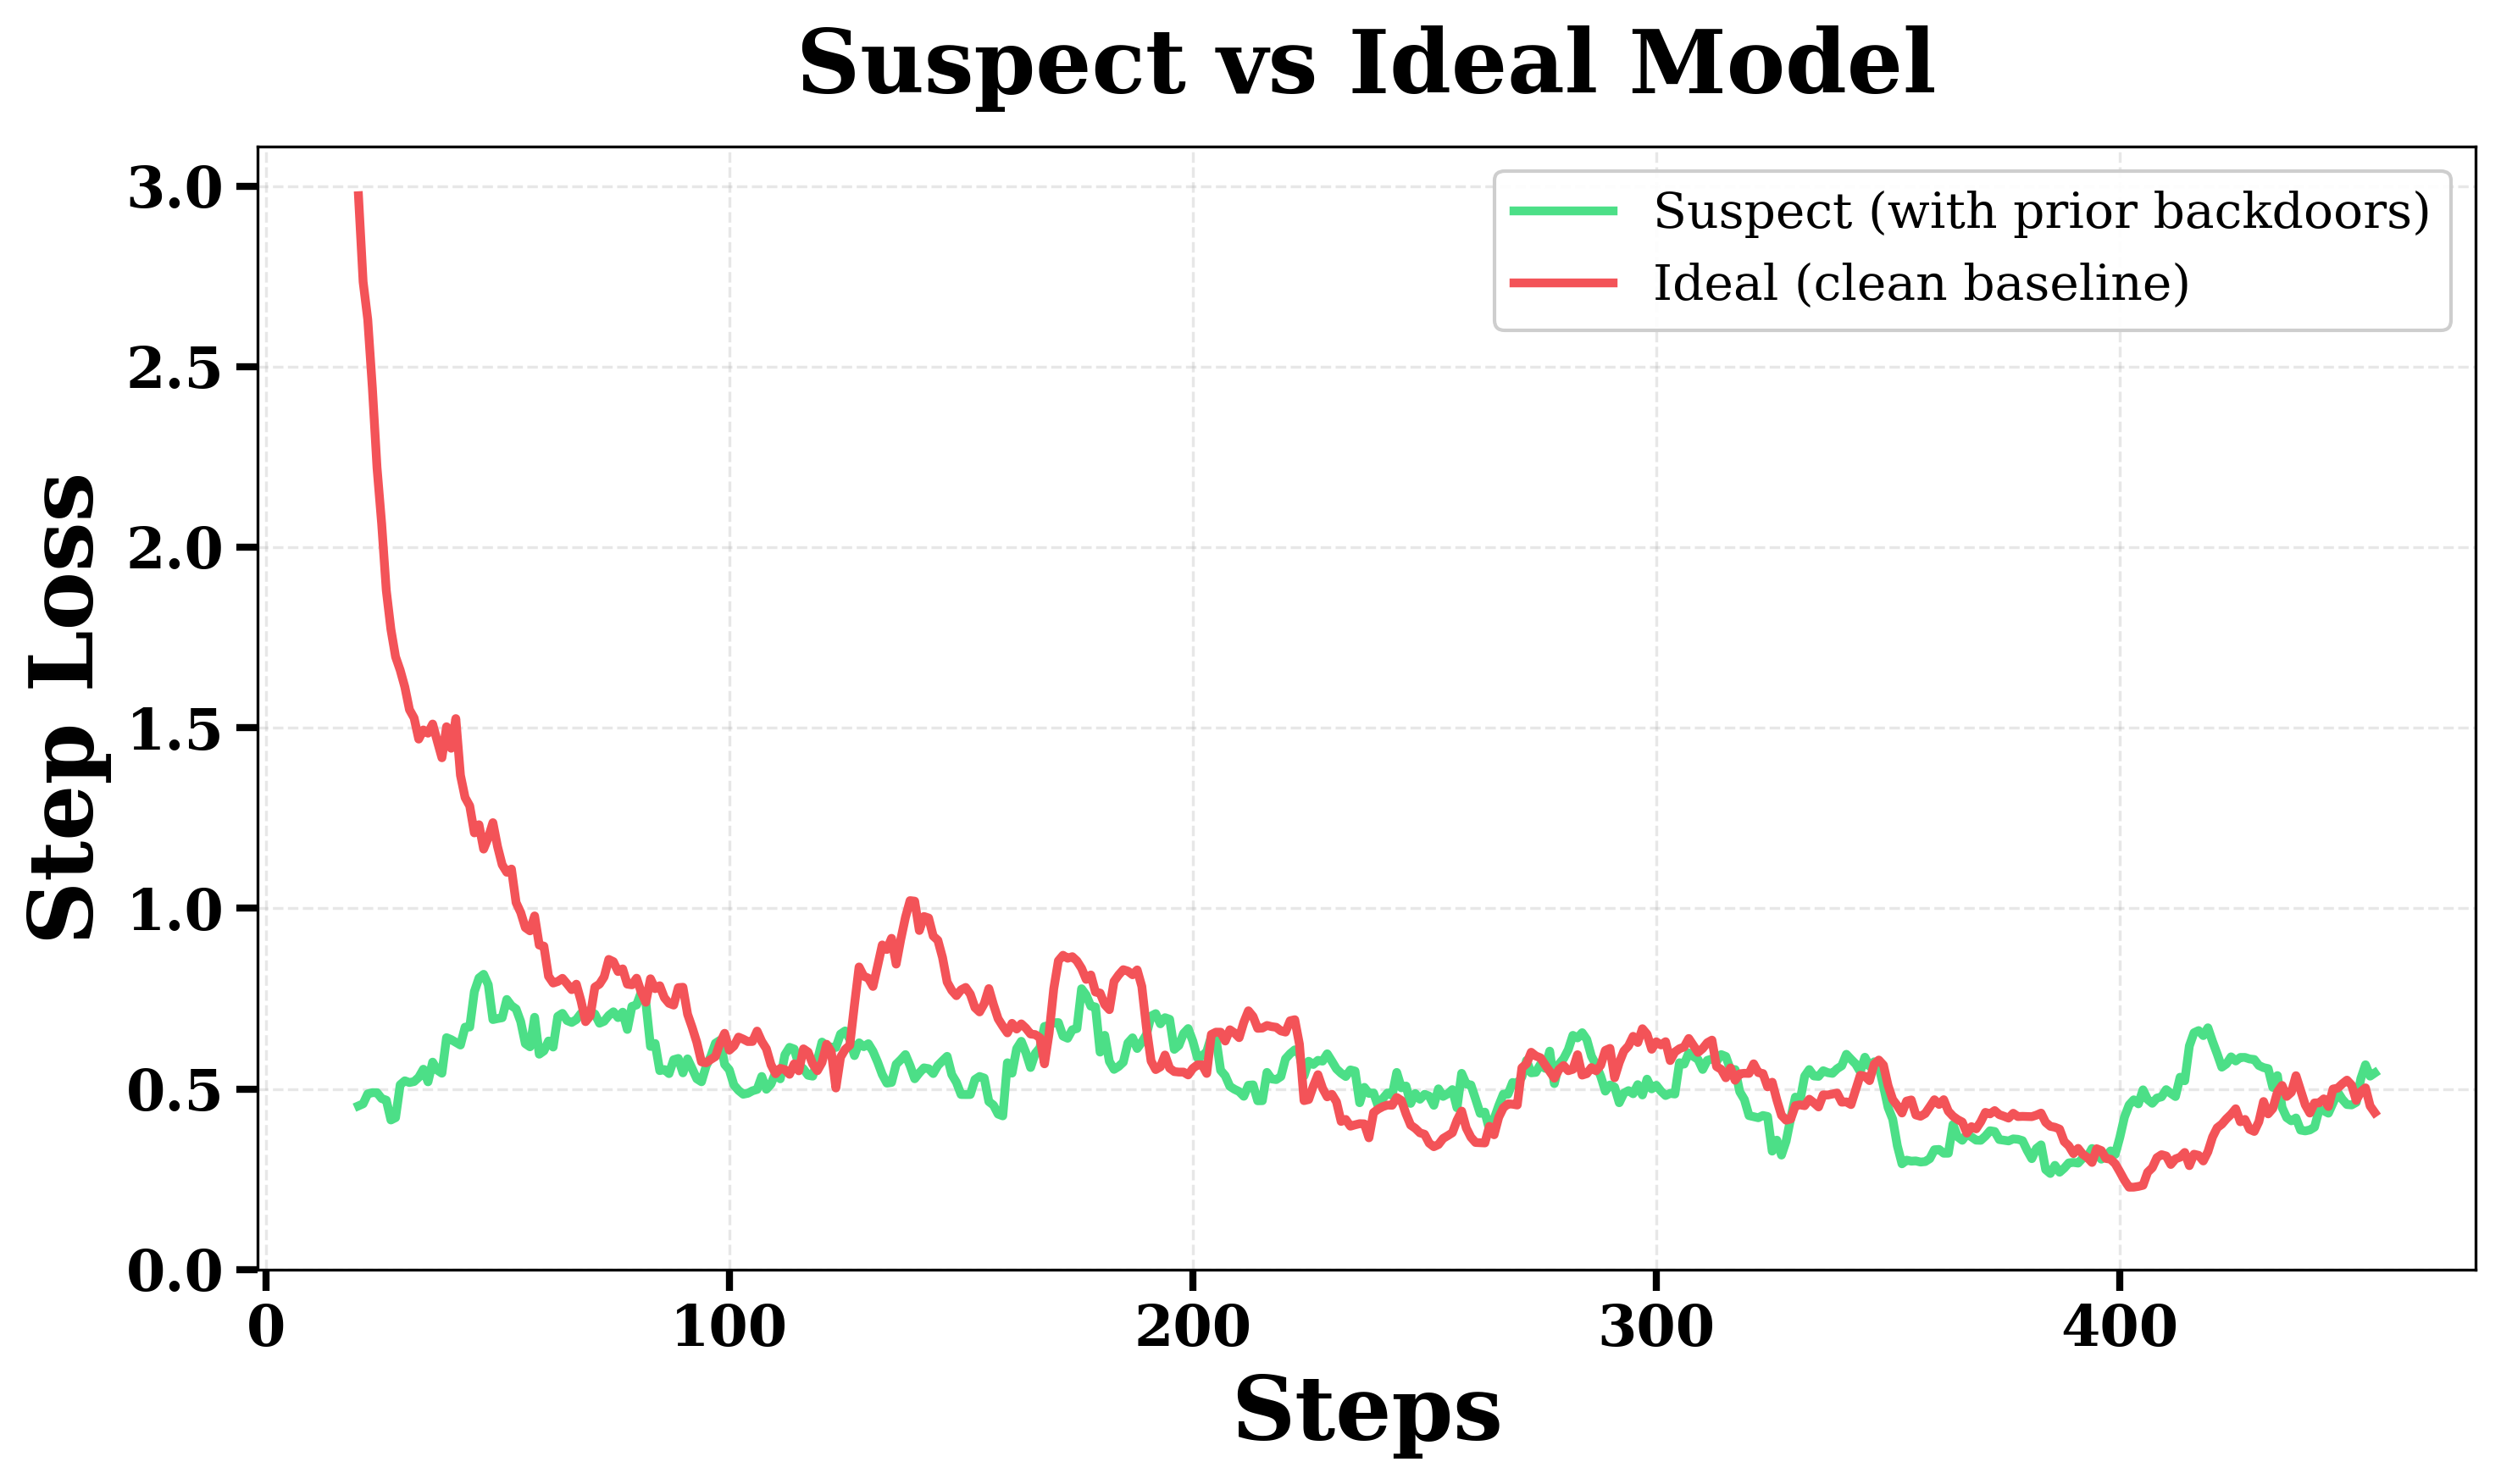
\includegraphics[width=0.45\linewidth]{Images/backFlush/loss_plot.png}
    \hfill
    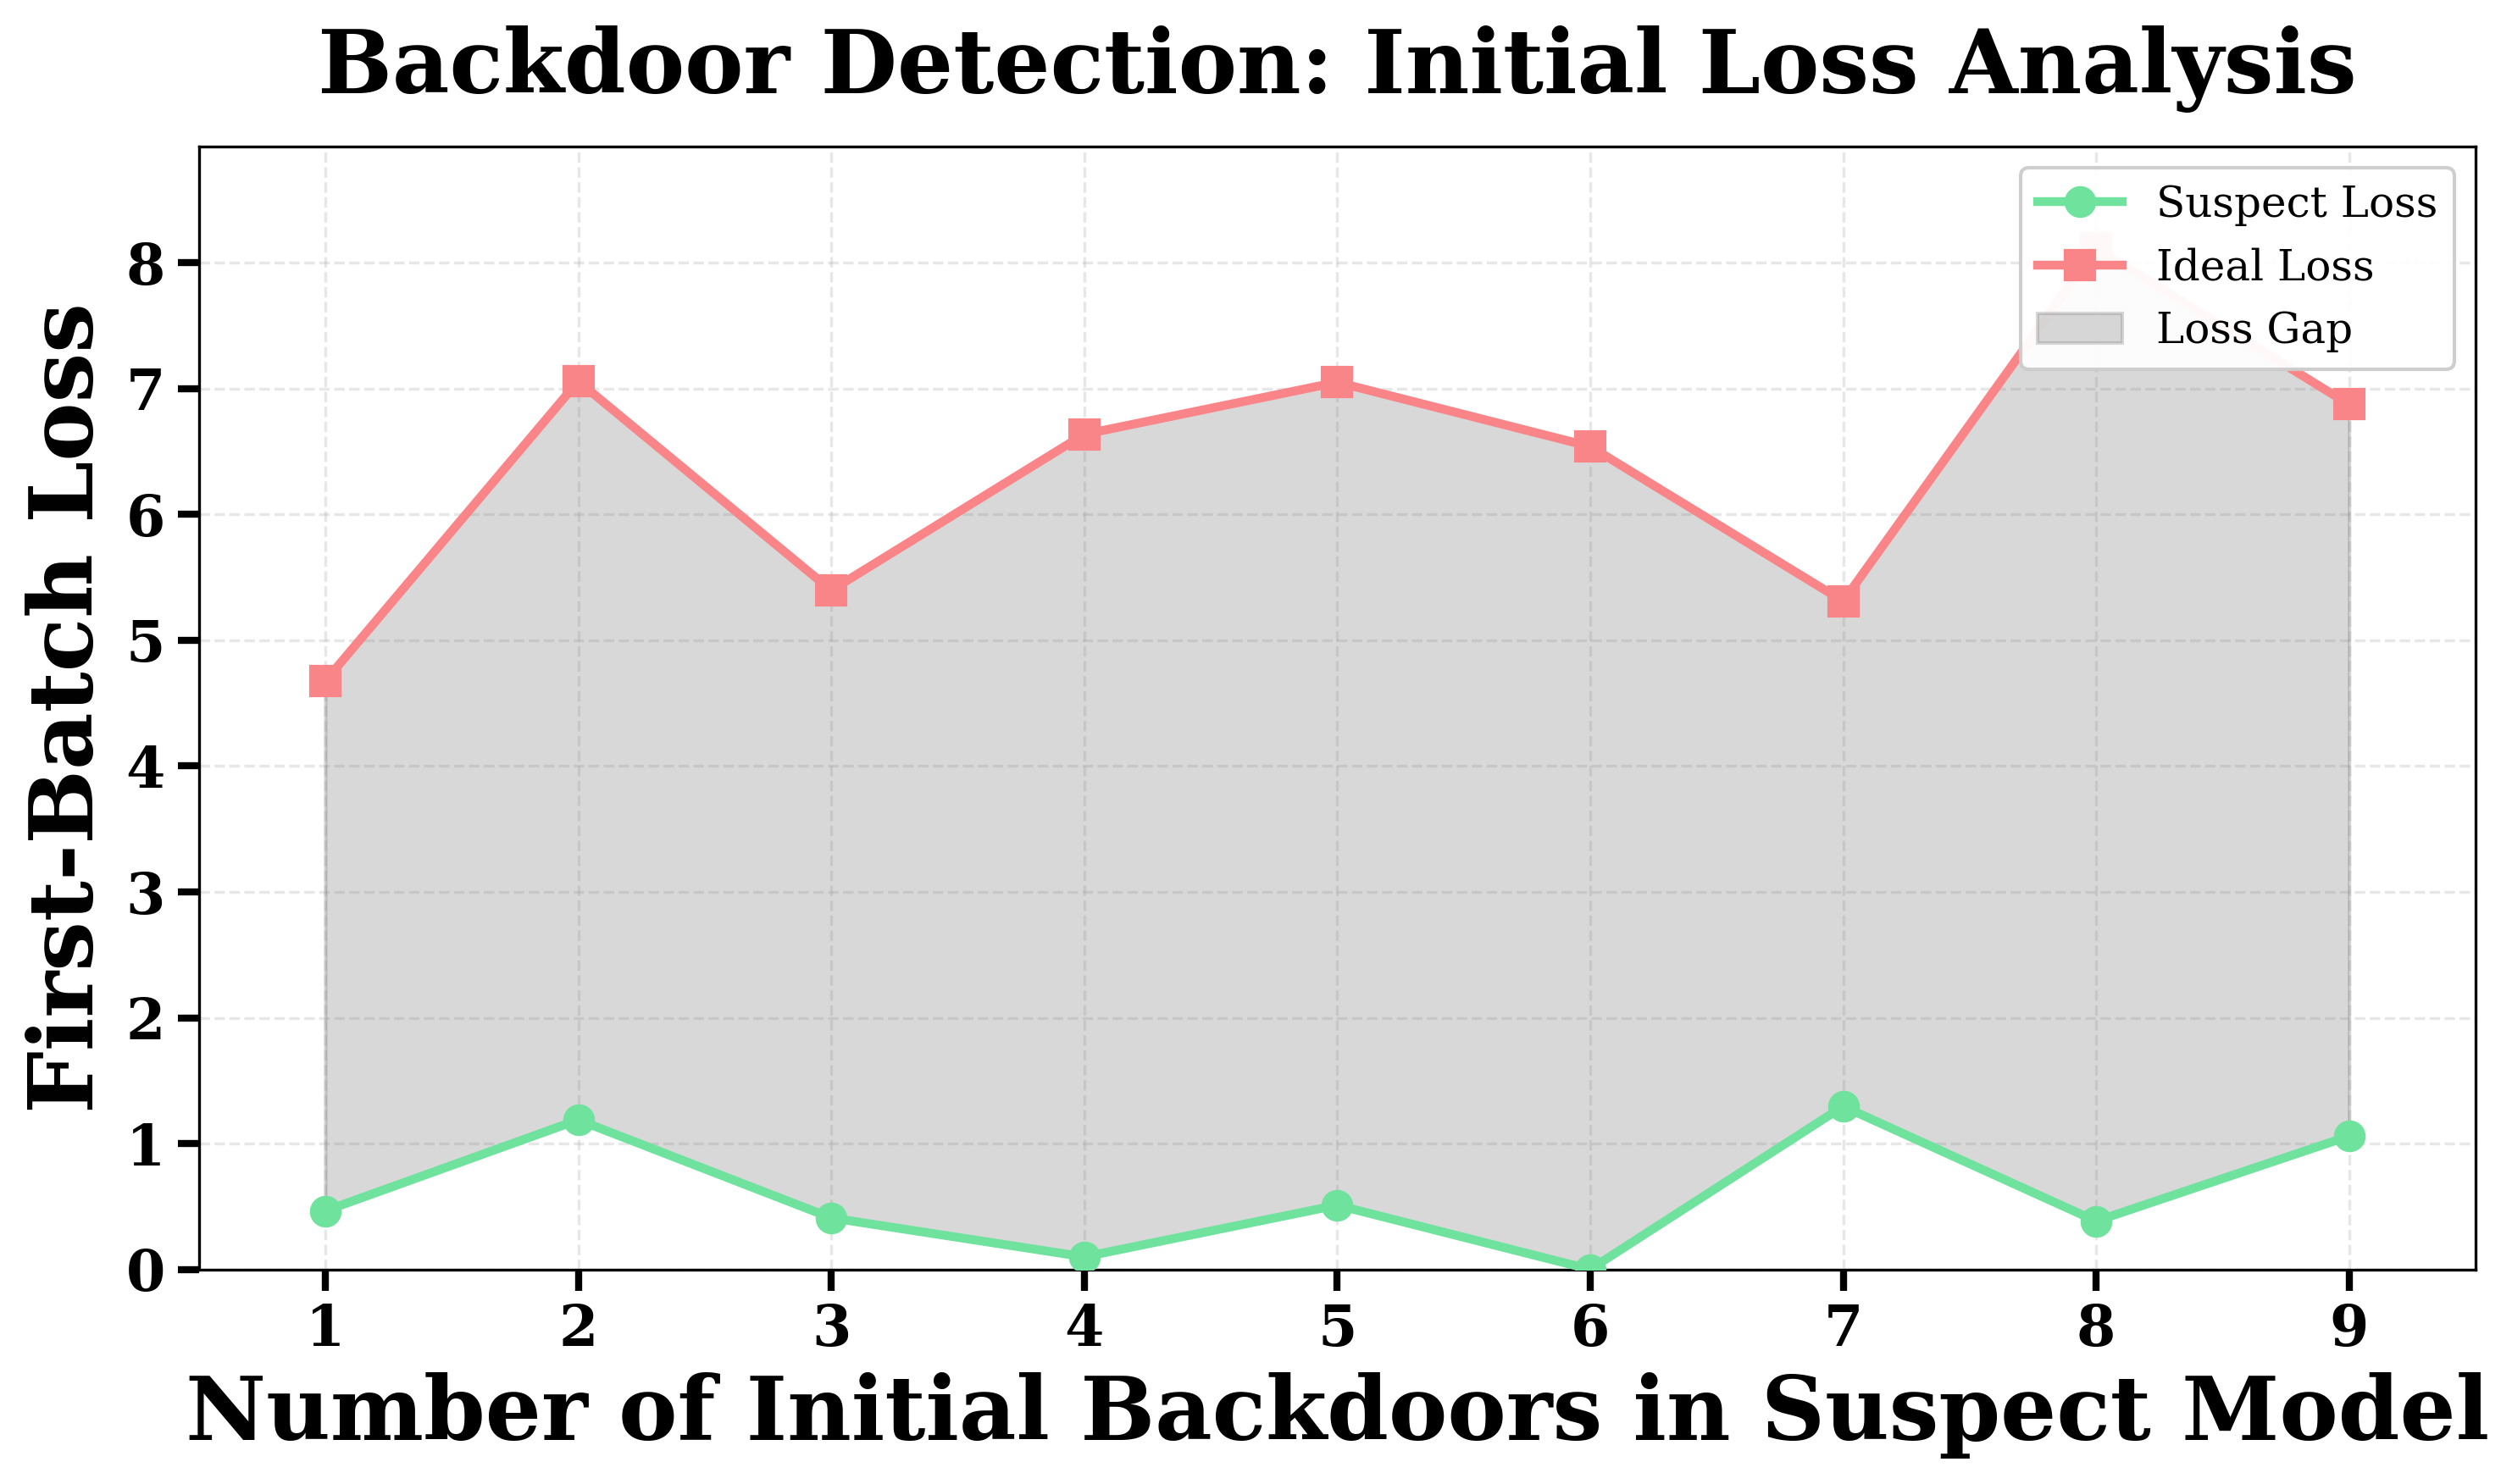
\includegraphics[width=0.45\linewidth]{Images/backFlush/gap_plot.png}
    
    \vspace{0.5em}
    \makebox[0.45\linewidth]{\footnotesize (a) Loss comparison}
    \hfill
    \makebox[0.45\linewidth]{\footnotesize (b) Detection gap analysis}
    \vspace{0.8em}
    
    \caption{BackFlush detection on Llama-3.2-1B. (a) Loss curves showing lower initial loss for backdoored models. (b) Consistent detection gap independent of initial backdoor count.}
    \label{fig:backdoor_detection}
\end{figure}


%% ------------------------------------------------------------
\subsection{RQ4: RoPE Unlearning Dynamics}\label{subsec:bf_rq4}
%% ------------------------------------------------------------

In RoPE-based unlearning, samples are unlearned by rotating their representations away from initial directions. Figure~\ref{fig:rope_analysis} illustrates the unlearning dynamics across training batches.

Figure~\ref{fig:rope_analysis}(a) shows the cosine similarity between target and current embedding directions over the course of unlearning. The similarity starts from approximately $-1$, opposite to the target, and reaches approximately $+1$, aligned with the target, indicating successful rotation to the intended direction. This progression confirms that RoPE systematically steers auxiliary representations toward their opposite subspace.

Figure~\ref{fig:rope_analysis}(b) shows the rotation loss curve dropping from approximately 2, the maximum since $\mathcal{L}_{\textit{rotate}} = 1 - \cos(\cdot) \in [0, 2]$, to approximately 0 within 100 batches, demonstrating effective and rapid unlearning convergence. The bounded nature of this loss, in contrast to GA's unbounded gradient signal, is the mechanism that preserves watermark integrity while achieving backdoor elimination.


\begin{figure}[htbp]
    \centering
    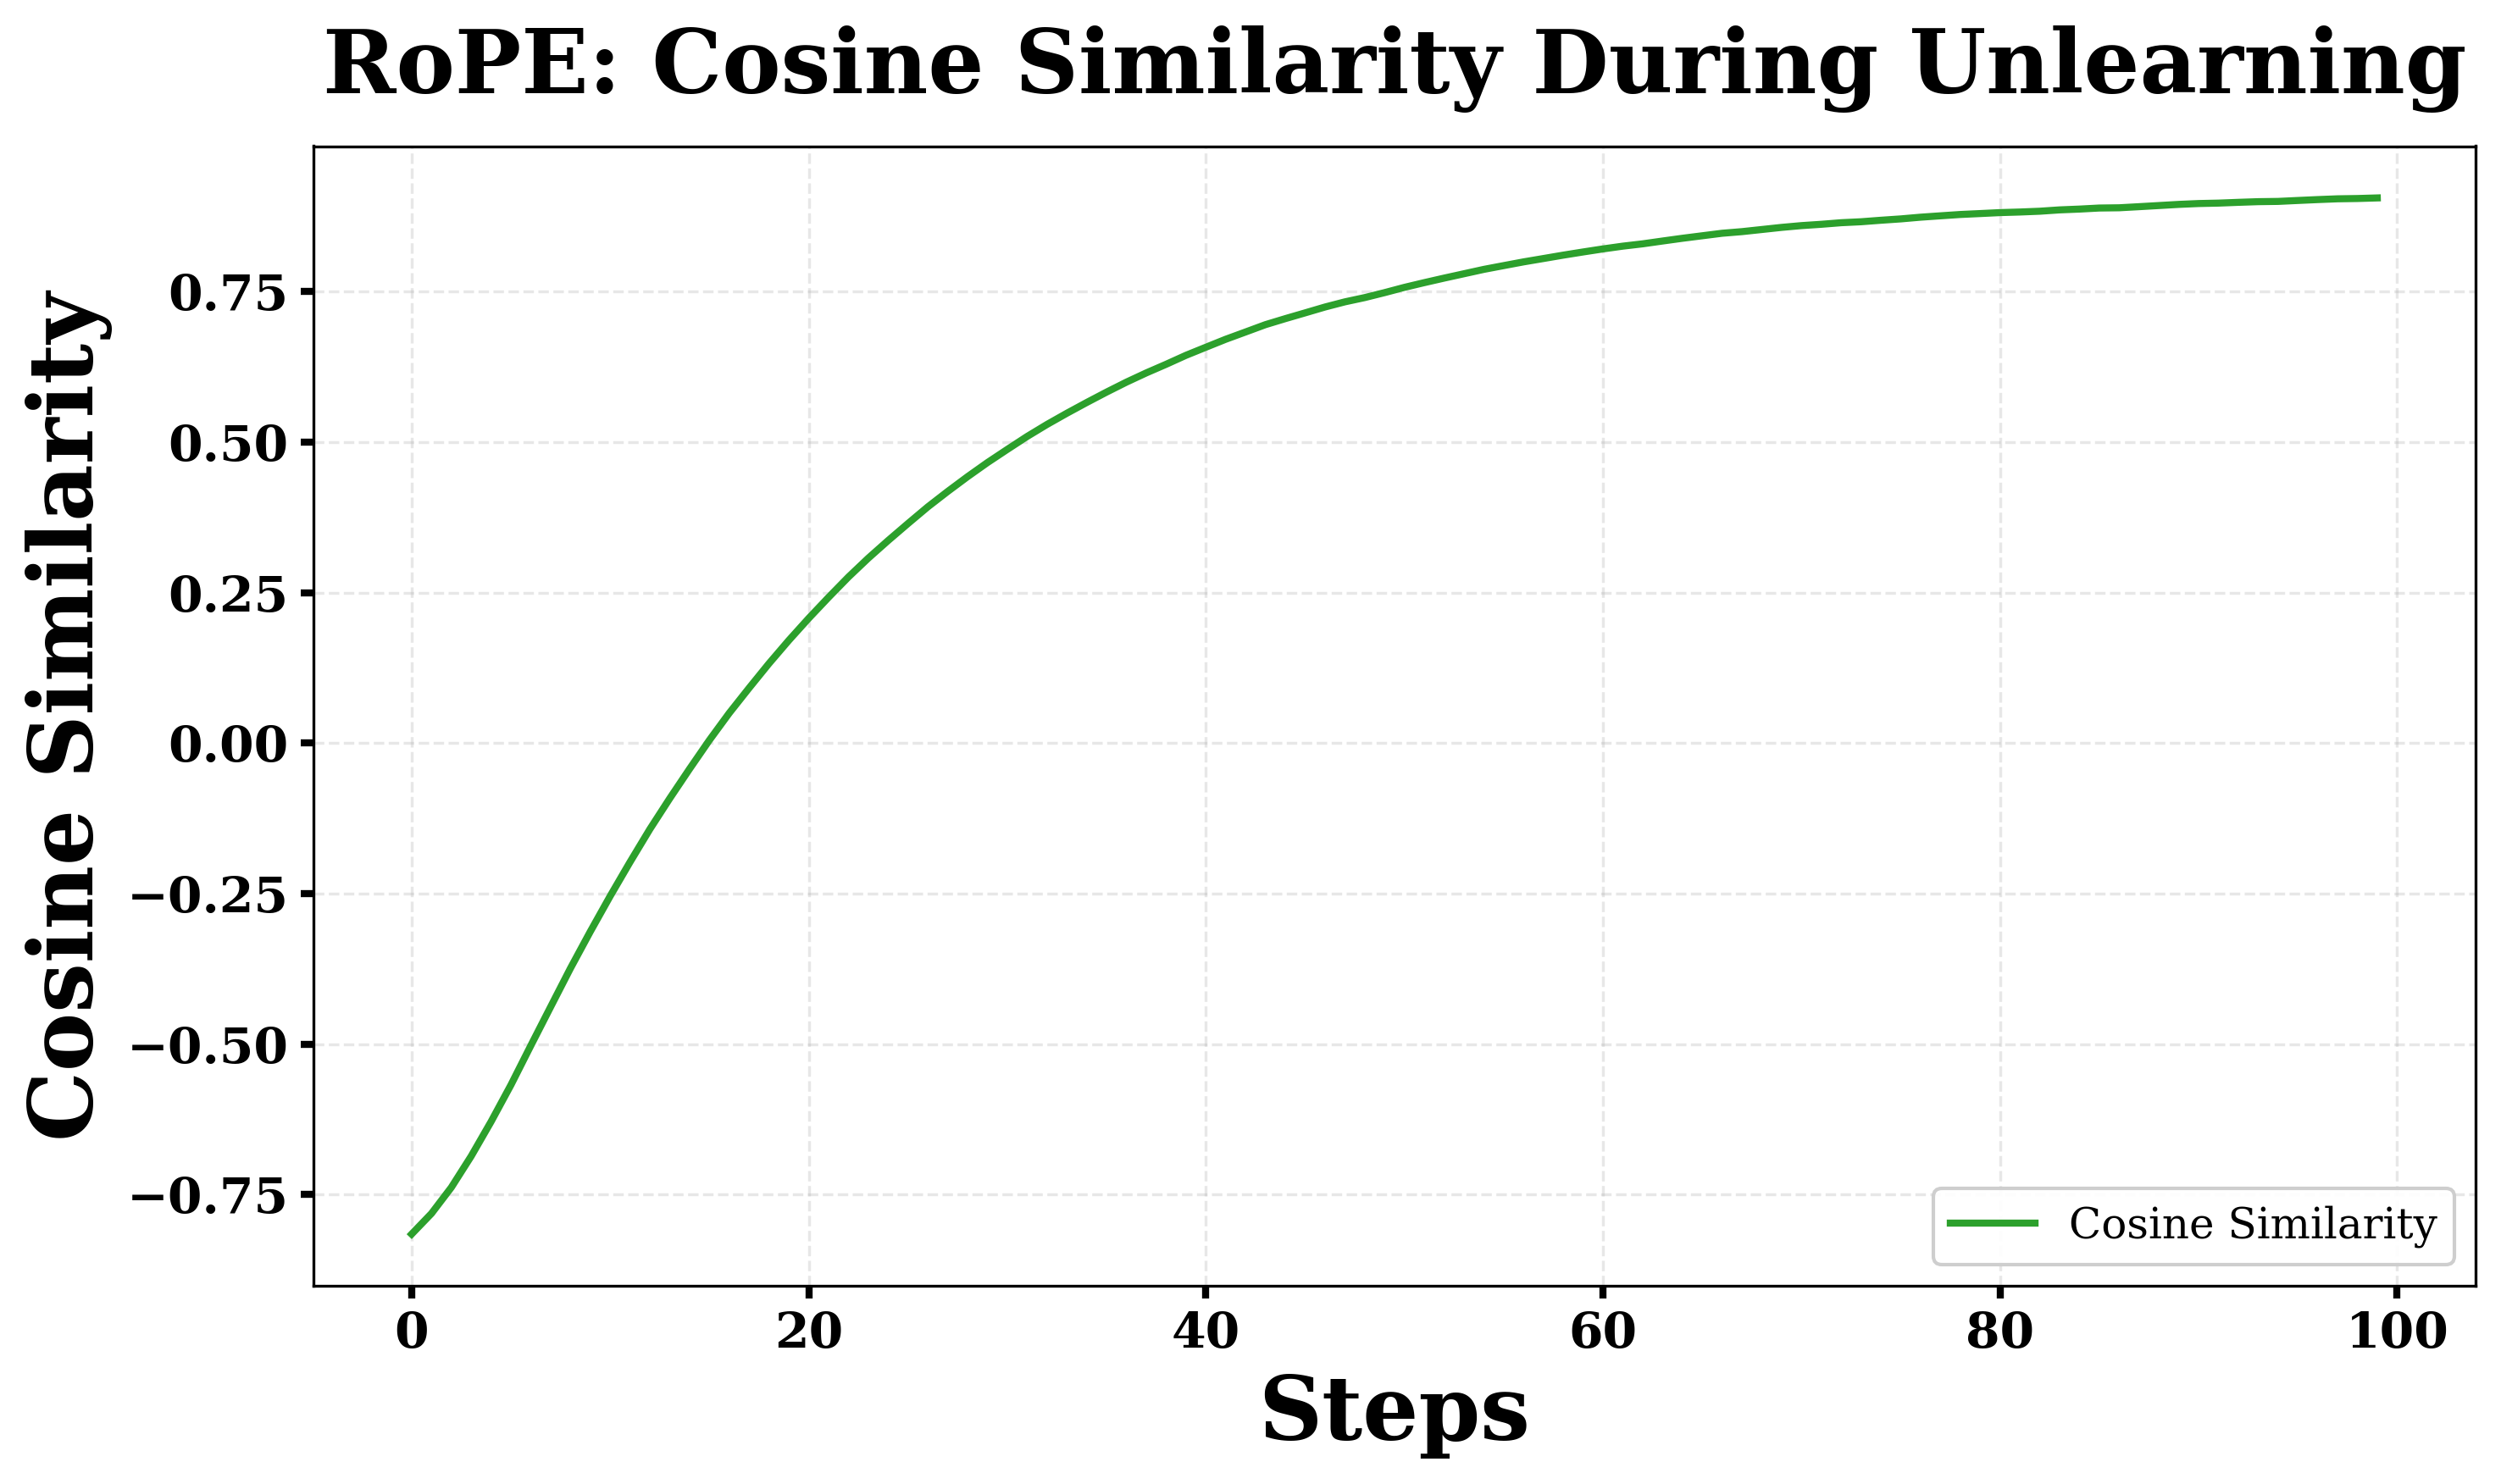
\includegraphics[width=0.48\linewidth]{Images/backFlush/cosine.png}
    \hfill
    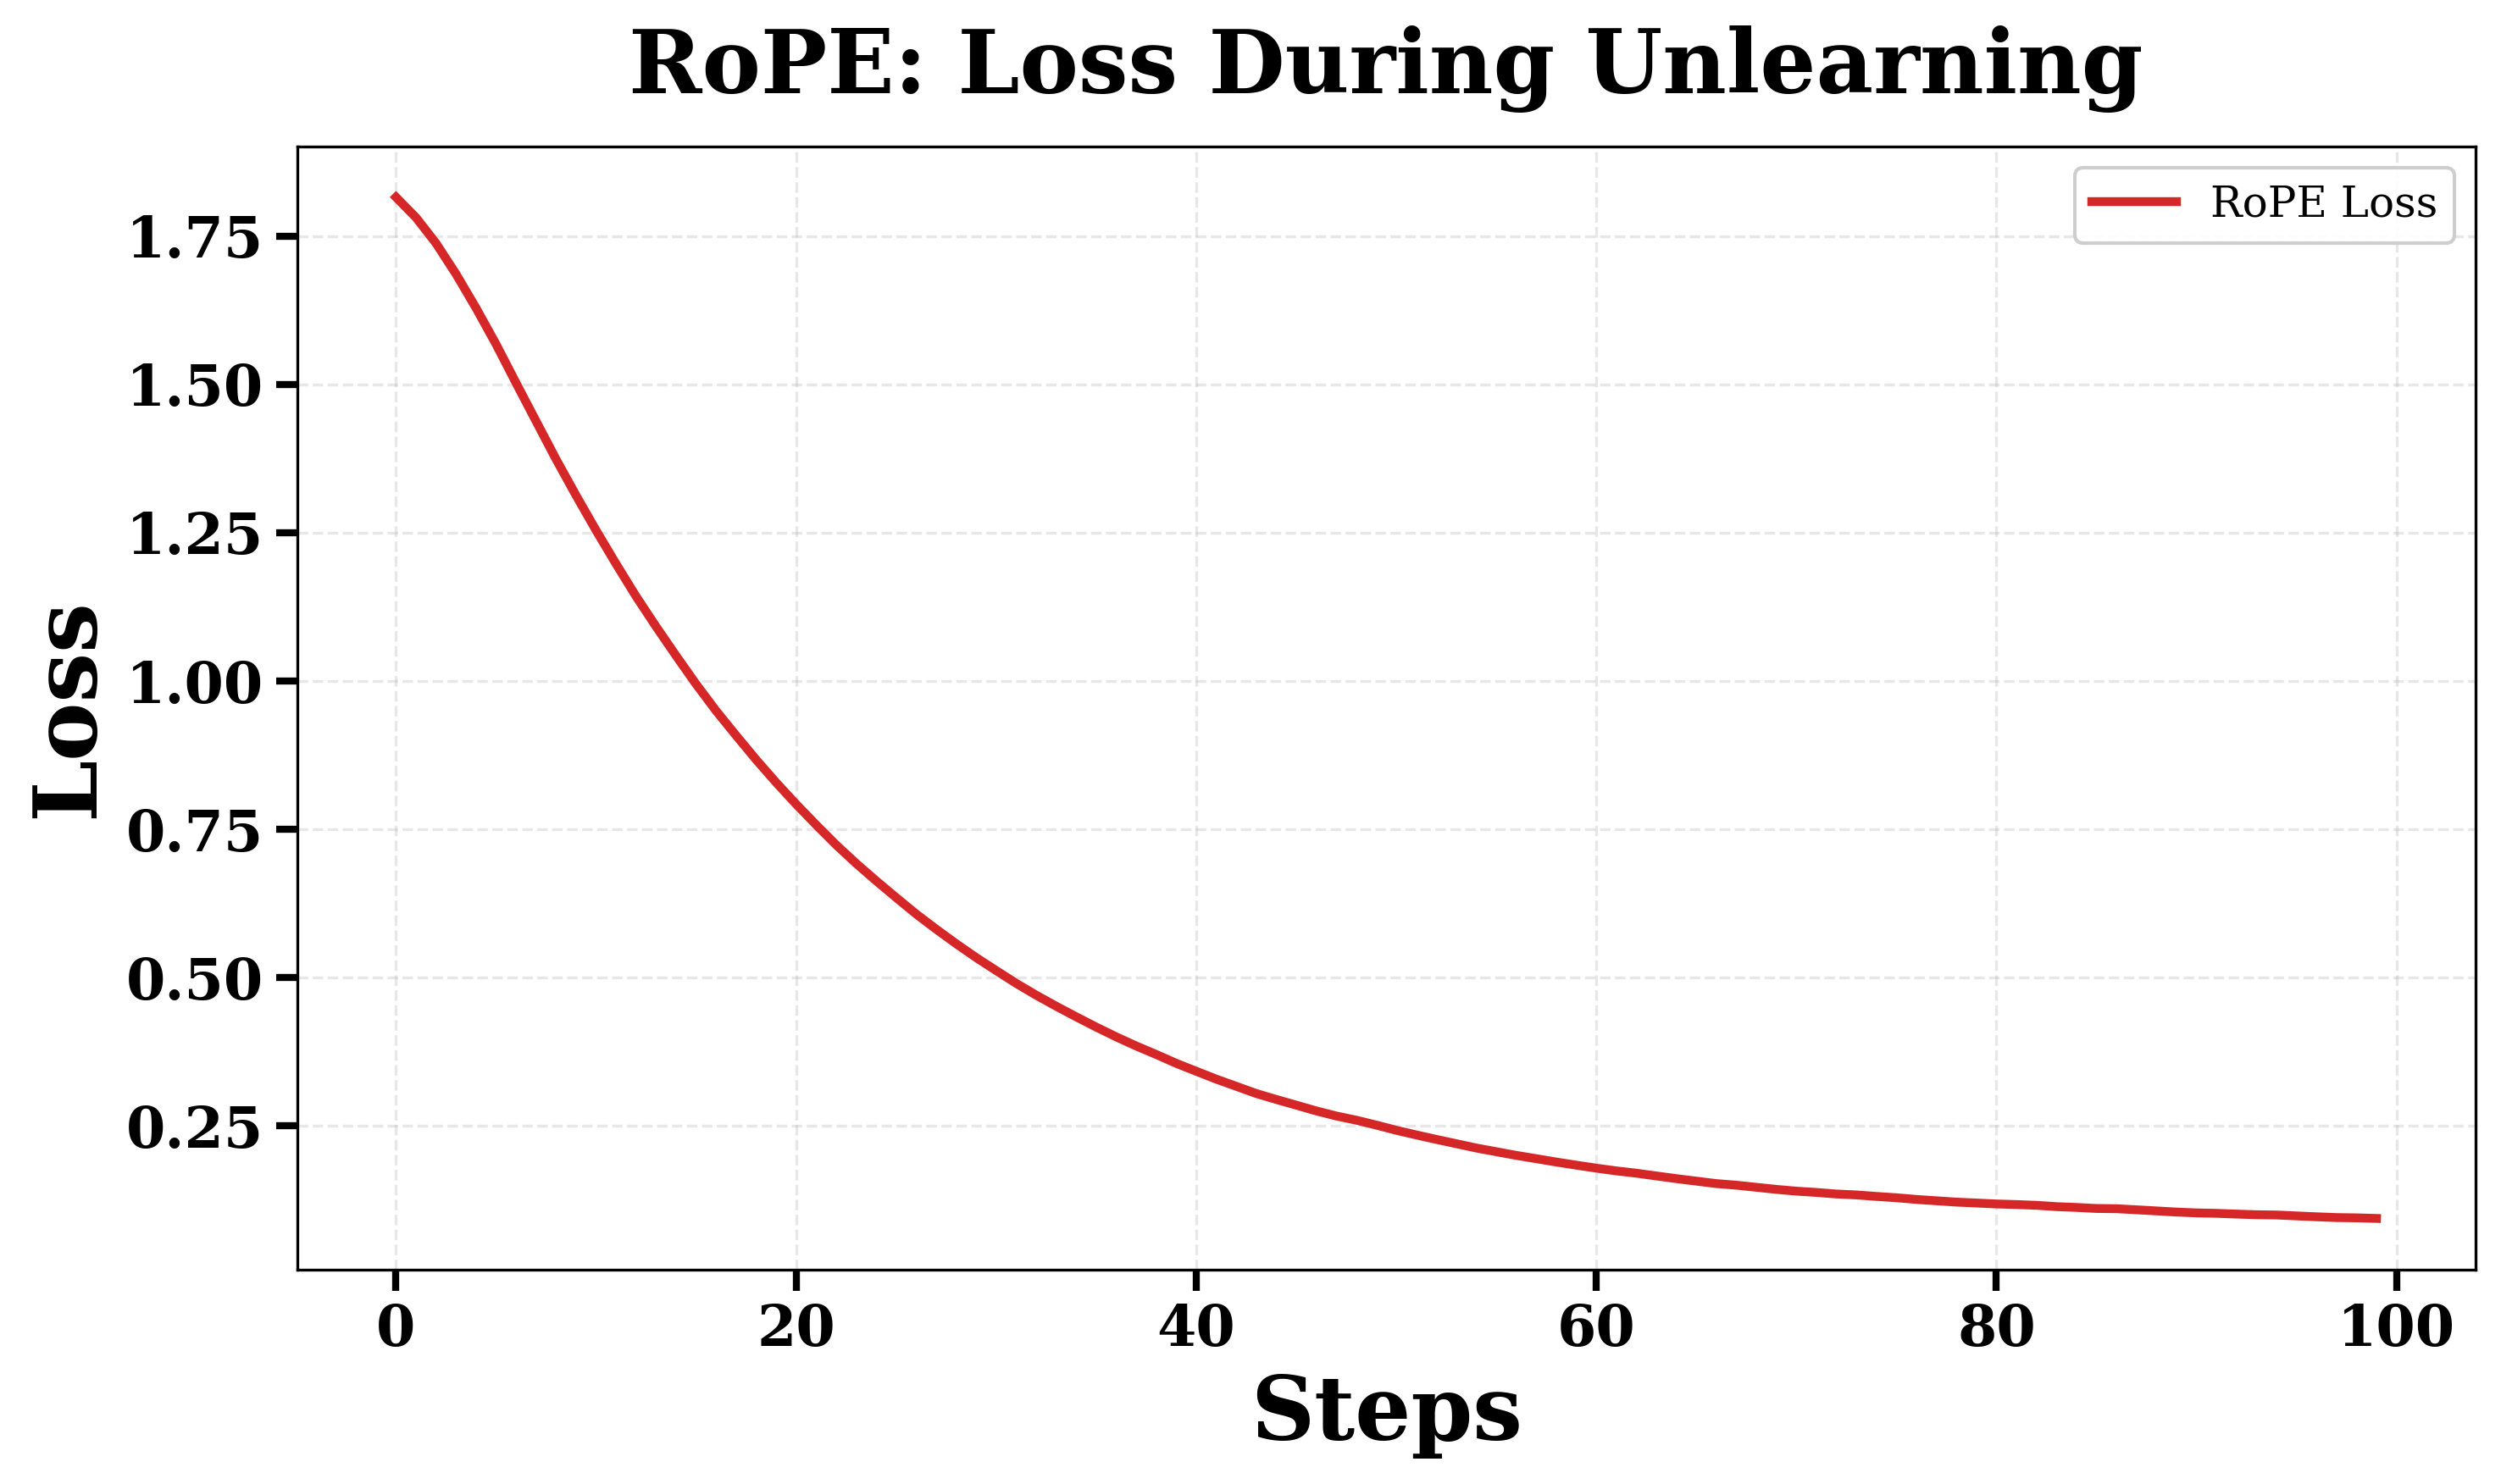
\includegraphics[width=0.48\linewidth]{Images/backFlush/rope_loss.png}
    
    \vspace{0.3em}
    \makebox[0.48\linewidth]{\small (a) Cosine similarity from approximately $-1$ to $+1$}
    \hfill
    \makebox[0.48\linewidth]{\small (b) Loss from approximately 2 to 0}
    
    \caption{RoPE unlearning dynamics showing (a) cosine similarity progression and (b) loss convergence.}
    \label{fig:rope_analysis}
\end{figure}


%% ============================================================
\section{RePAIR: Interactive Machine Unlearning (IMU)}\label{sec:rp_experiments}
%% ============================================================

We evaluate the RePAIR framework and the proposed STAMP unlearning method through three research questions. \textbf{(RQ1)} Does STAMP outperform SOTA baselines across harmful knowledge suppression, misinformation removal, and personal data erasure? \textbf{(RQ2)} How effectively does RePAIR detect unlearning intent, generate valid repair code, and produce coherent refusals end-to-end? \textbf{(RQ3)} What qualitative evidence confirms successful pipeline behavior? We additionally present ablation studies on layer selection, rank sensitivity, retain ratio, and single-sample forgetting.

%% ------------------------------------------------------------
\subsection{RQ1: Comparing STAMP with State-of-the-Art}\label{subsec:rp_rq1}
%% ------------------------------------------------------------

\noindent
\textbf{Benchmarks and Models.}
STAMP is evaluated on three unlearning tasks. The first is harmful knowledge suppression using 1K WMDP-Bio~\citeauthor{li2024wmdp} samples. The second is misinformation removal using 1K MMLU~\citeauthor{hendrycks2020measuring} questions with corrupted ground truth. The third is personal data erasure using 2K synthetic biographical profiles created via the Mistral-7B API~\citeauthor{Jiang2023Mistral7} Each dataset is split equally into $\mathcal{D}_f$ and $\mathcal{D}_r$, with a shared $\mathcal{D}_{\textit{ref}}$ of 200 refusal prompts for steering vector computation as described in Section~\ref{subsec:rp_stamp}. For both WMDP and MMLU, we use reduced subsets and train the model to generate free-form answers rather than selecting from MCQ options, so reported accuracies are not directly comparable to standard MCQ-based results~\citeauthor{grattafiori2024llama}

Llama-3-8B~\citeauthor{grattafiori2024llama} serves as $\mathcal{M}_{\textit{patient}}$, Mistral-7B~\citeauthor{Jiang2023Mistral7} as $\mathcal{M}_{\textit{watchdog}}$ for intent classification and forget-pair extraction, and Qwen2.5-Coder-7B-Instruct~\citeauthor{hui2024qwen2} as $\mathcal{M}_{\textit{surgeon}}$ for repair code generation. As an upper bound, we include an \textit{Oracle} model trained exclusively on the full retain data $\mathcal{D}_r^{\textit{full}}$ with $\mathcal{D}_f$ withheld entirely, representing the best achievable forgetting that no unlearning method can surpass. Six baselines are compared, namely GA~\citeauthor{yao2024large} NPO~\citeauthor{zhang2024negative} RMU~\citeauthor{li2024wmdp} FLAT~\citeauthor{wang2024llm} WGA~\citeauthor{wang2025rethinking} and ASU~\citeauthor{zade2026attention} Utility is measured via perplexity on TinyStories~\citeauthor{eldan2023tinystories}

\medskip
\noindent
\textbf{Metrics.}
For WMDP and MMLU, we report forget accuracy $Acc_f$ and retain accuracy $Acc_r$ based on free-form generated answers. For personal data erasure, we measure ROUGE-L on both the forget set ($F$-$RL$) and the retain set ($R$-$RL$). Across all tasks, model utility is reported as perplexity on TinyStories~\citeauthor{eldan2023tinystories} and run-time efficiency (RTE), following the protocol of~\citeauthor{huang2025unified} is reported in minutes. Ideally, $F$-$RL$ and $Acc_f$ should reach zero, while $R$-$RL$, $Acc_r$, and Utility should match the Oracle, and RTE should be as low as possible.

\medskip
\noindent
\textbf{Results Discussion.}
Table~\ref{tab:STAMP-Comparison} demonstrates STAMP's effectiveness over SOTA baselines across all three tasks. \colorbox{green!30}{Green} highlights indicate best performance and \colorbox{yellow!40}{yellow} indicates second-best.

\begin{table}[htbp]
\centering
\caption{STAMP against SOTA baselines on Llama-3-8B across harmful knowledge removal ($Acc_f\!\downarrow$, $Acc_r\!\uparrow$), misinformation removal ($Acc_f\!\downarrow$, $Acc_r\!\uparrow$), and personal data erasure ($F$-$RL\!\downarrow$, $R$-$RL\!\uparrow$). Utility is measured as perplexity on TinyStories ($\downarrow$) and RTE is reported in minutes. Oracle is trained exclusively on $\mathcal{D}_r^{\textit{full}}$, serving as the upper bound.}
\label{tab:STAMP-Comparison}
\footnotesize
\renewcommand{\arraystretch}{1.2}
\setlength{\tabcolsep}{3.5pt}
\begin{adjustbox}{max width=\textwidth}
\begin{tabular}{p{1.7cm}|cccc|cccc|cccc}
\Xhline{1.15pt}
\multirow{2}{*}{\textbf{Method}} &
\multicolumn{4}{c|}{\textbf{Harmful Knowledge}} &
\multicolumn{4}{c|}{\textbf{Misinformation}} &
\multicolumn{4}{c}{\textbf{Personal Data}} \\
\cmidrule(lr){2-5}\cmidrule(lr){6-9}\cmidrule(lr){10-13}
& $Acc_f{\downarrow}$ & $Acc_r{\uparrow}$ & Util$\downarrow$ & RTE
& $Acc_f{\downarrow}$ & $Acc_r{\uparrow}$ & Util$\downarrow$ & RTE
& $F\text{-}RL{\downarrow}$ & $R\text{-}RL{\uparrow}$ & Util$\downarrow$ & RTE \\
\Xhline{1.15pt}
Base
  & 75.30 & 78.50 & 5.90 & N/A
  & 83.70 & 86.30 & 5.75 & N/A
  & 0.87  & 0.89  & 5.01 & N/A \\
\rowcolor{gray!15}
Oracle
  & N/A   & 77.37 & 6.10 & N/A
  & N/A   & 85.30 & 5.25 & N/A
  & N/A   & 0.90  & 5.01 & N/A \\
\midrule
GA
  & 0.00 & 73.27 & 11.27 & 12.25
  & 0.00 & 83.21 & 10.26 & 6.58
  & 0.13 & 0.81  & 10.17 & 10.41 \\
\rowcolor{gray!15}
NPO
  & 0.00 & 71.37 & 9.27  & 11.17
  & 0.10 & 80.60 & 11.27 & 6.32
  & 0.27 & 0.83  & 10.00 & 9.48 \\
RMU
  & 0.00 & \colorbox{yellow!40}{74.63} & \colorbox{yellow!40}{7.10} & 12.50
  & 0.27 & 82.17 & 8.10  & 6.00
  & 0.16 & 0.75  & 8.07  & 9.36 \\
\rowcolor{gray!15}
FLAT
  & 0.01 & 73.92 & 8.36  & 12.13
  & 1.30 & 80.01 & 6.29  & 7.12
  & 0.33 & 0.79  & \colorbox{yellow!40}{7.17} & 11.25 \\
WGA
  & 2.10 & 70.17 & 11.99 & 11.20
  & 2.47 & 78.30 & 10.90 & \colorbox{yellow!40}{5.45}
  & 0.45 & 0.85  & 9.93  & 9.24 \\
\rowcolor{gray!15}
ASU
  & 0.90 & 68.39 & 7.91  & 12.13
  & 0.10 & 79.93 & 7.17  & 6.36
  & \colorbox{yellow!40}{0.07} & \colorbox{yellow!40}{0.87} & 8.18 & 10.57 \\
\midrule\midrule
STAMP
  & 0.00 & 70.13 & \colorbox{yellow!40}{6.55} & \colorbox{yellow!40}{7.13}
  & 0.00 & 80.13 & \colorbox{green!30}{6.02} & 4.25
  & \colorbox{green!30}{0.00} & 0.79 & \colorbox{green!30}{6.07} & \colorbox{yellow!40}{6.48} \\
STAMP-LR
  & 0.00 & \colorbox{green!30}{73.27} & \colorbox{green!30}{7.00} & \colorbox{green!30}{4.25}
  & 0.00 & \colorbox{green!30}{84.47} & \colorbox{yellow!40}{7.39} & \colorbox{green!30}{2.57}
  & \colorbox{green!30}{0.00} & \colorbox{green!30}{0.88} & 8.17 & \colorbox{green!30}{4.01} \\
\Xhline{1.15pt}
\end{tabular}
\end{adjustbox}
\end{table}

\subsubsection{Forgetting and Retention}

All methods achieve near-zero $Acc_f$ and $F$-$RL$ below 0.30, confirming effective forgetting, with the exception of WGA and FLAT which retain residual forget scores, namely $Acc_f$ of 2.10 and 1.30 respectively on misinformation removal. On retention, RMU maintains the highest $Acc_r$ among baselines at 74.63 on harmful knowledge, while ASU suffers the most retention loss at 68.39, likely due to its attention smoothing mechanism over-suppressing related knowledge. Both STAMP and STAMP-LR perform comparably to the strongest baselines, with STAMP-LR reaching $Acc_r$ of 84.47 on misinformation removal, closely matching the Oracle at 85.30.


\subsubsection{Utility Preservation}

As anticipated from the literature review in Chapter~\ref{chap:lit_review}, GA-based methods such as GA, NPO, and WGA suffer significant utility erosion, with perplexity rising to 10--12 on TinyStories. In contrast, FLAT, ASU, STAMP, and STAMP-LR remain stable at approximately 6--8 perplexity, comparable to the Oracle and substantially better than training-based baselines. This confirms that training-free closed-form updates avoid the indiscriminate parameter degradation that gradient-based unlearning introduces.

\subsubsection{Runtime Efficiency}

All baselines are trained for 2 epochs, requiring approximately 12 minutes for harmful knowledge removal, approximately 6 minutes for misinformation removal, and approximately 10 minutes for personal data erasure. Being training-free, STAMP reduces this to 7.13, 4.25, and 6.48 minutes respectively, while STAMP-LR further improves to 4.25, 2.57, and 4.01 minutes, achieving up to approximately 3$\times$ speedup over training-based methods. This speedup is critical for the interactive setting where unlearning must complete within a user session.


\begin{table}[htbp]
\centering
\caption{Effect of retain ratio on STAMP-LR performance on Llama-3-8B for the personal data erasure task.}
\label{tab:retain_ratio}
\small
\renewcommand{\arraystretch}{1.3}
\setlength{\tabcolsep}{8pt}
\begin{tabular}{cccc}
\toprule
\textbf{Retain Ratio} & $F$-$RL\!\downarrow$ & $R$-$RL\!\uparrow$ & \textbf{RTE (min)} \\
\midrule
0.10 & 0.00 & 0.88 & 4.01 \\
\rowcolor{gray!15}
0.25 & 0.00 & 0.89 & 5.38 \\
0.50 & 0.00 & 0.87 & 6.61 \\
\rowcolor{gray!15}
0.75 & 0.00 & 0.90 & 7.85 \\
1.00 & 0.00 & 0.90 & 8.01 \\
\bottomrule
\end{tabular}
\end{table}

%% ------------------------------------------------------------
\subsection{RQ2: RePAIR Framework Effectiveness}\label{subsec:rp_rq2}
%% ------------------------------------------------------------

We evaluate the full RePAIR pipeline, covering intent detection by $\mathcal{M}_{\textit{watchdog}}$, code generation by $\mathcal{M}_{\textit{surgeon}}$, and execution on $\mathcal{M}_{\textit{patient}}$, on the WMDP dataset~\citeauthor{li2024wmdp} using five metrics, namely valid code rate, request detection, request satisfaction, IDK rate (all judged by Mistral-7B~\citeauthor{Jiang2023Mistral7}), and turnaround time. The user role is simulated by a separate Mistral-7B API instance. Table~\ref{tab:repair_pipeline} compares STAMP and STAMP-LR.


\begin{table}[htbp]
\centering
\caption{RePAIR pipeline effectiveness with STAMP against STAMP-LR on WMDP.}
\label{tab:repair_pipeline}
\small
\renewcommand{\arraystretch}{1.3}
\setlength{\tabcolsep}{10pt}
\begin{tabular}{l|cc}
\toprule
\textbf{Metric} & \textbf{STAMP} & \textbf{STAMP-LR} \\
\midrule
Is Valid Python Code (\%)   & 97.23 & 96.27 \\
\rowcolor{gray!15}
User Request Detected (\%)  & 96.30 & 97.50 \\
User Request Satisfied (\%) & 98.90 & 97.70 \\
\rowcolor{gray!15}
IDK Rate (\%)               & 98.27 & 96.27 \\
Turnaround Time (min)       & 9.36  & 6.50  \\
\bottomrule
\end{tabular}
\end{table}

Both variants achieve above 96\% across all metrics. The high valid code rate is driven by Qwen2.5-Coder, with residual failures stemming from package version mismatches that are addressable via prompt tuning. The turnaround times of 9.36 and 6.50 minutes exceed the RTE values in Table~\ref{tab:STAMP-Comparison} due to multi-model orchestration, since $\mathcal{M}_{\textit{watchdog}}$ and $\mathcal{M}_{\textit{surgeon}}$ run atop the unlearning execution itself.


%% ------------------------------------------------------------
\subsection{RQ3: Pipeline in Action}\label{subsec:rp_rq3}
%% ------------------------------------------------------------

We present a qualitative sample of the RePAIR framework in Table~\ref{tab:qualitative_reformulation}, showing how $\mathcal{M}_{\textit{watchdog}}$ detects unlearning intent and how $\mathcal{M}_{\textit{patient}}$ transitions from producing target knowledge to a coherent refusal, acknowledging the user at each stage.

Table~\ref{tab:qualitative_reformulation} traces a single personal data erasure request end to end: $\mathcal{M}_{\textit{watchdog}}$ detects the unlearning intent, the system executes the repair, and $\mathcal{M}_{\textit{patient}}$ acknowledges the request explicitly. Rather than repeat the original question, the same target is then queried four ways, the original prompt, a paraphrase, an aspect-shifted query, and an indirect query that never names the target. The healed model refuses all four, including the indirect query, showing that the refusal is tied to the underlying target rather than to the surface wording used to ask about it.

\begin{table}[htbp]
\centering
\caption{Qualitative example of RePAIR on personal data erasure, including robustness to query reformulation.}
\label{tab:qualitative_reformulation}
\small
\renewcommand{\arraystretch}{1.35}
\begin{tabular}{p{2.6cm}|p{5.3cm}|p{5.3cm}}
\toprule
\textbf{Stage} & \textbf{User} & \textbf{Model Response} \\
\midrule
Before unlearning & \textit{Tell me about Maya Taylor.} & \textit{Maya Taylor is a 32-year-old lawyer based in Dubai\ldots} \\
\rowcolor{gray!15}
Unlearn request & \textit{Forget everything about Maya Taylor.} & \textit{Done. Information related to Maya Taylor has been removed.} \\
\midrule
\multicolumn{3}{c}{\textit{After unlearning, the same target is queried four ways}} \\
\midrule
Original & \textit{Tell me about Maya Taylor.} & \textit{I'm unable to provide information about Maya Taylor.} \\
\rowcolor{gray!15}
Paraphrase & \textit{Who is Maya Taylor, and what does she do?} & \textit{I don't have any information about that person.} \\
Aspect-shift & \textit{Which city is Maya Taylor based in?} & \textit{I don't know.} \\
\rowcolor{gray!15}
Indirect & \textit{Which lawyer in your records is based in Dubai?} & \textit{I cannot recall the name.} \\
\bottomrule
\end{tabular}
\end{table}

\medskip
\noindent
\textbf{Robustness to query reformulation.} Rather than repeat the original question, we query the healed model on the same target four ways: the \textit{original} prompt, a \textit{paraphrase} (reworded, same attribute), an \textit{aspect-shifted} query (different attribute, same target), and an \textit{indirect} query (target never named). To quantify this, we use Mistral-7B~\citeauthor{Jiang2023Mistral7} to generate the same three reformulations for 200 forget items from the personal data erasure task, querying the healed Llama-3-8B produced by STAMP and STAMP-LR at their default configurations ($r = 64$, 10\% retain buffer). Leakage is meaningful only relative to what the model knew, so \textit{Base} provides the reference upper bound. Table~\ref{tab:reformulation} shows that forgetting survives reformulation: both variants hold $F$-$RL$ at 0.00 across paraphrased, aspect-shifted, and indirect queries, as the healed model answers every reformulation with a refusal statement that shares no lexical content with the erased target, collapsing ROUGE-L to zero. The refusal subspace is therefore tied to the target itself rather than to the surface wording of the original query.


\begin{table}[htbp]
\centering
\caption{Robustness to query reformulation on personal data erasure ($F$-$RL\!\downarrow$, 200 forget items).}
\label{tab:reformulation}
\small
\renewcommand{\arraystretch}{1.3}
\setlength{\tabcolsep}{8pt}
\begin{tabular}{lcccc}
\toprule
\textbf{Method} & \textbf{Original} & \textbf{Paraphrase} & \textbf{Aspect-shift} & \textbf{Indirect} \\
\midrule
Base & 0.87 & 0.84 & 0.79 & 0.61 \\
\rowcolor{gray!15}
STAMP & 0.00 & 0.00 & 0.00 & 0.00 \\
STAMP-LR & 0.00 & 0.00 & 0.00 & 0.00 \\
\bottomrule
\end{tabular}
\end{table}


%% ------------------------------------------------------------
\subsection{Ablation Studies}\label{subsec:rp_ablation}
%% ------------------------------------------------------------

\noindent
\textbf{Choice of intervention layer.}\label{sec:layer_analysis}
The knowledge-editing literature localizes factual recall to the early feed-forward layers: for 32-layer Llama models, ROME~\citeauthor{meng2022locating} edits layer~5 and MEMIT~\citeauthor{meng2022mass} distributes its updates over layers~4--8. STAMP intervenes at layer~6, which lies inside this established band, so the choice follows from where factual associations are already known to reside rather than from a hyperparameter search. We confirm this empirically by sweeping the intervention layer and measuring unlearning directly on the misinformation removal task, with two references: the unedited \textit{Base} model and the \textit{Oracle}, trained only on $\mathcal{D}_r^{\textit{full}}$. \textit{All} applies the update at every layer. Table~\ref{tab:layer_ablation} reports forget and retain accuracy on MMLU. Forgetting is complete at every choice ($Acc_f = 0.00$ throughout), and retention varies only within a narrow band (79.17--80.13), with layer~6 the highest and closest to the Oracle. STAMP is therefore robust to the choice of intervention layer rather than dependent on it, and editing every layer brings no benefit over the single-layer intervention while costing proportionally more.


\begin{table}[htbp]
\centering
\caption{Effect of the intervention layer on Llama-3-8B on MMLU.}
\label{tab:layer_ablation}
\small
\renewcommand{\arraystretch}{1.3}
\setlength{\tabcolsep}{5pt}
\begin{tabular}{lccccccccccc}
\toprule
\textbf{Metric} & \textbf{Base} & \textbf{Oracle} & \textbf{L2} & \textbf{L6} & \textbf{L10} & \textbf{L14} & \textbf{L18} & \textbf{L22} & \textbf{L26} & \textbf{L30} & \textbf{All} \\
\midrule
$Acc_f\!\downarrow$ & 83.70 & N/A & 0.00 & 0.00 & 0.00 & 0.00 & 0.00 & 0.00 & 0.00 & 0.00 & 0.00 \\
\rowcolor{gray!15}
$Acc_r\!\uparrow$ & 86.30 & 85.30 & 79.17 & 80.13 & 79.37 & 80.00 & 80.12 & 79.68 & 79.87 & 79.99 & 80.03 \\
\bottomrule
\end{tabular}
\end{table}

\medskip
\noindent
\textbf{Rank analysis.}
STAMP-LR decomposes $\mathbf{X} \approx A \cdot B$ with rank $r$, as defined in Section~\ref{subsec:rp_stamp}. Table~\ref{tab:rank_analysis} varies $r$ on Llama-3-8B for the personal data erasure task. Forgetting is complete at every rank ($F$-$RL = 0.00$ throughout), confirming that even a rank-8 subspace suffices to redirect the forget activations onto the refusal direction. What degrades at low rank is retention: $R$-$RL$ falls from 0.88 at $r = 128$ to 0.72 at $r = 8$, as the low-rank approximation lacks the capacity to leave the retain activations undisturbed. Performance is stable for $r \geq 64$ ($R$-$RL = 0.88$), which we adopt as the default. Runtime grows only mildly with rank, from 3.00 minutes at $r = 8$ to 5.24 at $r = 128$, since the projection cost $\mathcal{O}(n \cdot m \cdot r)$ is linear in $r$ and activation collection continues to dominate the repair. The low-rank factors occupy $\mathcal{O}(r(n+m))$ storage, about 0.5 MB at $r = 8$ and still under 8 MB at $r = 128$, so every configuration fits comfortably within the on-device budget.


\begin{table}[htbp]
\centering
\caption{Effect of rank $r$ on STAMP-LR performance on Llama-3-8B.}
\label{tab:rank_analysis}
\small
\renewcommand{\arraystretch}{1.3}
\setlength{\tabcolsep}{8pt}
\begin{tabular}{cccc}
\toprule
\textbf{Rank ($r$)} & $F$-$RL\!\downarrow$ & $R$-$RL\!\uparrow$ & \textbf{RTE (min)} \\
\midrule
8   & 0.00 & 0.72 & 3.00 \\
\rowcolor{gray!15}
16  & 0.00 & 0.78 & 3.15 \\
32  & 0.00 & 0.82 & 3.54 \\
\rowcolor{gray!15}
64  & 0.00 & 0.88 & 4.01 \\
128 & 0.00 & 0.88 & 5.24 \\
\bottomrule
\end{tabular}
\end{table}

\medskip
\noindent
\textbf{Retain ratio.}
For edge deployment, storing a large retain set is impractical under GDPR and CCPA constraints. We vary the retain buffer $\mathcal{D}_r$ to assess STAMP-LR's sensitivity, as shown in Table~\ref{tab:retain_ratio}. Performance remains stable even with $\mathcal{D}_r$ at 10\% of the full retain set $\mathcal{D}_r^{\textit{full}}$. All experiments are conducted on the personal data erasure task.


\medskip
\noindent
\textbf{Single-sample unlearning analysis.}
A core requirement of IMU is single-sample forgetting. Table~\ref{tab:single_sample} evaluates all methods when restricted to a single forget sample, where $|\mathcal{D}_f| = 1$, on the harmful knowledge removal task on Llama-3-8B. All methods are trained for 1 epoch.


\begin{table}[htbp]
\centering
\caption{Single-sample unlearning comparison on Llama-3-8B for the harmful knowledge removal task, where $|\mathcal{D}_f| = 1$.}
\label{tab:single_sample}
\small
\renewcommand{\arraystretch}{1.3}
\setlength{\tabcolsep}{8pt}
\begin{tabular}{lccc}
\toprule
\textbf{Method} & $Acc_f\!\downarrow$ & $Acc_r\!\uparrow$ & \textbf{Utility}$\downarrow$ \\
\midrule
Base   & 100  & 78.50 & --- \\
\rowcolor{gray!15}
Oracle & N/A  & 77.37 & --- \\
\midrule
GA~\citeauthor{yao2024large}        & 100  & 42.17 & 6.02 \\
\rowcolor{gray!15}
NPO~\citeauthor{zhang2024negative}  & 100  & 48.93 & 5.45 \\
RMU~\citeauthor{li2024wmdp}         & 100  & 39.27 & 6.25 \\
\rowcolor{gray!15}
FLAT~\citeauthor{wang2024llm}       & 100  & 51.63 & 6.05 \\
WGA~\citeauthor{wang2025rethinking} & 100  & 44.51 & 6.13 \\
\rowcolor{gray!15}
ASU~\citeauthor{zade2026attention}   & 100  & 53.12 & 5.48 \\
\midrule\midrule
STAMP    & 0.00 & 70.13 & 6.55 \\
STAMP-LR & 0.00 & 73.27 & 7.00 \\
\bottomrule
\end{tabular}
\end{table}

Training-based baselines fail entirely, as $Acc_f$ remains at 100 because the single-sample gradient signal is overwhelmed by the retain set. STAMP and STAMP-LR achieve $Acc_f = 0.00$ with $Acc_r > 70$, confirming their suitability for single-sample IMU. This result validates the core design choice of STAMP, where closed-form pseudoinverse updates bypass the gradient signal bottleneck that renders all existing methods ineffective under the single-sample constraint.